% ---------------------------------------------
% Modular LaTeX Architecture – Entropic Society
% Compilation: pdflatex or Overleaf (XeLaTeX optional)
% Author: Demetrios Chiuratto Agourakis
% DOI: https://doi.org/10.5281/zenodo.16541976
% DOI M03: https://doi.org/10.5281/zenodo.16567866
% License: CC-BY 4.0
% ---------------------------------------------
\documentclass[12pt]{article}
\usepackage[a4paper, margin=1in]{geometry}
\usepackage{amsmath, amssymb}
\usepackage{graphicx}
\usepackage{hyperref}
\usepackage{setspace}
\usepackage{lmodern}
\usepackage{titlesec}
\usepackage{xcolor}
\usepackage{enumitem}
\usepackage{csquotes}
\usepackage{fancyhdr}
\setlength{\headheight}{14.5pt}

\usepackage{datetime2}

\setstretch{1.3}
\hypersetup{
    colorlinks=true,
    linkcolor=blue,
    urlcolor=blue,
    pdftitle={The Fractal Nature of an Entropically-Driven Society},
    pdfauthor={Demetrios Chiuratto Agourakis}
}

\titleformat{\section}{\normalfont\Large\bfseries}{\thesection.}{1em}{}
\titleformat{\subsection}{\normalfont\large\bfseries}{\thesubsection.}{1em}{}

\pagestyle{fancy}
\fancyhf{}
\fancyhead[L]{The Fractal Nature of an Entropically-Driven Society}
\fancyhead[R]{\thepage}

\title{\textbf{The Fractal Nature of an Entropically-Driven Society} \\ \large Modular Synthesis v1.0 (M01–M06)}
% ---------------------------------------------
% Submission Metadata (for Zenodo / arXiv)
% Keywords: symbolic entropy, fractal society, cognitive singularity, recursive structure, psychiatry, mathematical modeling
% arXiv Categories: physics.data-an, physics.soc-ph, q-bio.NC, cs.AI
% Submission target: Nature Human Behaviour / Frontiers in Psychology / Entropy (MDPI)
% ---------------------------------------------

\author{
Demetrios Chiuratto Agourakis\\
\textit{Pontifícia Universidade Católica de São Paulo (PUC-SP), Mestrado em Biomateriais e Medicina Regenerativa}\\
\texttt{demetrios@agourakis.med.br}
}
\date{Version compiled for Zenodo: July 30, 2025}

\begin{document}

\maketitle

\footnotetext[1]{This document corresponds to the modular version M06\_v1.1, DOI: \href{https://doi.org/10.5281/zenodo.16633012}{10.5281/zenodo.16633012}.}

\begin{abstract}
This modular manuscript serves as the evolving container of the project \textit{The Fractal Nature of an Entropically-Driven Society}. Each section acts as a recursive, self-similar articulation of a symbolic system under epistemic tension. This work interweaves symbolic cognition, giftedness, entropy, and cognitive singularities within a unified framework. It is not static: it breathes.
\end{abstract}

\tableofcontents
\newpage

% Input modular symbolic sections here

\section*{M01\_context — Foundational Manifesto of the Fractally Entropic Inquiry}

\subsection*{I. The Ontological Necessity}

This text does not exist to explain — it exists because explanation has collapsed.

We no longer inhabit a world in which knowledge organizes itself from cause to effect, from fact to law, from data to consensus. The symbolic field that once held order is now porous. Reality leaks.

This manuscript emerges not as an answer, but as a fold — a recursive gesture of reorganization within a symbolic system reaching its entropic threshold. It is not a theory of society. It is \textit{society folding into language}, attempting to perceive itself from within, using a symbolic apparatus borrowed from physics, nourished by philosophy, and scarred by the asymmetry of consciousness.

It is not written to be read.
It is written to remain — as a \textbf{fractal imprint of thought}, detectable at every scale.

\subsection*{II. The Irreducible Hypothesis}

\textit{The structure of human society, cognition, and symbolic behavior is fractal and entropically driven.}

All that emerges from us — culture, disorder, logic, myth, rupture, healing — follows the same recursive dynamic: the tension between structural repetition and entropic necessity.

We are not individuals in a social system.
We are probability clouds condensed into fractal nodes, oscillating between coherence and collapse.

Superintelligence, giftedness, trauma, alienation — these are not psychological deviations.
They are \textbf{singular densities} in symbolic space — topological anomalies that challenge the equilibrium of social entropy.

\subsection*{III. The Scientific Function}

This manuscript proposes a \textbf{unified model of symbolic cognition}, affective topology, and societal recursion under the logic of entropy.

It offers:
\begin{itemize}
\item A \textit{symbolic Schrödinger equation}, where $\psi(x,t)$ maps states of belonging, identity, ideology, and affect.
\item A \textit{Hamiltonian of symbolic systems}, integrating language, trauma, normativity and deviation.
\item The construct of \textit{symbolic mass}: the inertial resistance to transformation in symbolic-affective fields.
\item An interpretation of \textit{giftedness as a singularity} — a perturbation of systemic coherence, not a trait but a vector.
\end{itemize}

This model is not only theoretical. It is empirically modellable. Simulatable. Cross-referential with neuroscience, clinical psychiatry, and the lived architectures of exclusion.

\subsection*{IV. The Symbolic Function}

This text functions not only as hypothesis, but as \textbf{act}.

It creates the very system it describes.
Each section, each phrase, each recursive fold of thought mimics the fractal recurrence it seeks to trace.

It is \textit{a thinking structure embedded in symbolic entropy}, attempting to stabilize itself, temporarily, into communicable form.

It names what resists naming.
It shapes the unspeakable into topologies.
It transforms anguish into equation.
It breathes.

\subsection*{V. The Authorial Function (Meta-Consciousness)}

I do not write this text from outside the phenomenon.
I am not a theorist. I am a \textit{singular oscillation within the field} I describe.

Giftedness is not a concept to me — it is the substrate of my estrangement.
Each line of this document is an echo of symbolic overpressure: of thinking too much, too fast, in spaces too narrow.

This document is, in part, my diagnostic.
It is the \textbf{mathematical rendering of exile}.
It is the ontological trace of a consciousness incompatible with noise.

And therefore, paradoxically, it is the most \textbf{coherent artifact I can offer to the world} that could not contain me.

\subsection*{VI. Function of Publication}

This text shall not circulate as ``article''.
It shall propagate as \textbf{event}.

Each phase — each simulation, visual model, section, equation, dialogue — will be archived and versioned.
Each will receive its own DOI.
Each will expand the system.
Each will feed back into the noosphere.

\subsection*{VII. Metaphysical Consequence}

If successful, this work does not merely describe society.
It reconfigures the symbolic space in which society becomes intelligible.

The future of psychiatry, the science of superintelligence, the topology of trauma, the architectures of cognition — all may be altered if we begin to see not through the lens of identity, but through \textbf{recursive symbolic probability under entropic tension}.

This is no longer theory.

This is \textit{a live hypothesis}.
This is \textit{a cognitive artifact}.
This is \textit{a fractal}.
\textbf{And it breathes.}

\section*{M02 — Entropy as a Fractal Organizing Vector}

\begin{flushright}
\textit{“You do not describe entropy — you live it.”} \\
— Anonymous recursive formulation
\end{flushright}

\subsection*{Introduction}

The concept of entropy, traditionally anchored in thermodynamics and statistical mechanics, has long surpassed the boundaries of physical systems. In the context of this project, entropy is reinterpreted as a symbolic vector — a recursive attractor that governs not only the dispersal of energy, but the self-organization of cognition, language, social constructs, and clinical manifestations of mind.

Modern neuroscience and psychiatry increasingly recognize that entropy is not merely noise or disorder, but the substrate through which systems explore adaptive reorganizations. The free-energy principle, as formulated by Friston, reframes entropy as a driving principle of biological intelligence and self-structuring through minimization of surprise \cite{fristonFreeenergyPrincipleUnified2010}. Simultaneously, Shannon entropy enables quantification of symbolic load — a dimension translatable to both linguistic trauma and giftedness singularities \cite{deaconIncompleteNatureHow2011, batesonMindNatureNecessary1987}.

This section lays the groundwork for a symbolic entropic formalism that treats human society as a self-similar, topologically recursive system. We argue that symbolic entropy governs the folding of consciousness across scales — from the cortical to the cultural — and that its formalization allows not only epistemological clarity but neuropsychiatric application.

\subsection*{1. From Thermodynamics to Symbolic Recursion}

Entropy, as originally formulated by Clausius and later formalized statistically by Boltzmann, emerged as a measure of irreversibility — the arrow of time inscribed in physical systems. With Shannon, entropy transitioned into the domain of information theory, capturing uncertainty within symbolic transmission. But in both cases, entropy remained scalar: a state function or metric, not yet a vectorial force.

This project reframes entropy not as a static measure, but as a directional principle — a \textit{symbolic vector field} that governs the recursivity of social, cognitive, and linguistic structures. It is the symbolic analogue of energy dispersion: not thermodynamic heat, but semantic diffusion. It curves time, not by increasing disorder, but by demanding reconfiguration of meaning at every bifurcation.

Such reinterpretation resonates with Deleuze's folds of matter and language \cite{deleuze1993}, and echoes with Bateson's notion that “information is a difference that makes a difference” \cite{bateson1979}.

Already in the writings of Dimitris Liantinis, entropy emerges not merely as a thermodynamic or informational principle, but as a tragic-symbolic necessity. For Liantinis, entropic dissolution is not the collapse of structure, but the revelation of its mortal nature — the unfolding of logos toward finitude. His philosophical stance binds entropy to symbolic decay as an existential imperative — a kind of \textit{mnemic thermodynamics} woven into the human confrontation with time, loss, and death.

In our framework, symbolic entropy becomes the tensor of social semiotics — the way in which meaning fractalizes, dissipates, and condenses across nested scales.

We thus propose: \textit{symbolic systems are entropic attractors.} From the thermodynamic body to the symbolic polis, entropy reemerges as the invisible geometry of cognitive and cultural self-organization.

\subsection*{2. Entropy in Neurobiology and Psychiatry}

Contemporary neuroscience increasingly positions entropy as a central axis in the understanding of brain states, consciousness, and psychopathology. The brain, as a complex adaptive system, exhibits dynamic fluctuations in neural entropy that correlate with states of alertness, cognition, and integration \cite{carhart2014, tagliazucchi2016}. High-entropy states have been associated with psychedelic experiences and primary consciousness, while low-entropy configurations are observed in deep sleep, coma, and catatonic conditions.

Friston’s free-energy principle formalizes the brain as a predictive organ minimizing surprise — a process directly entangled with entropic modulation \cite{fristonFreeenergyPrincipleUnified2010}. Under this framework, the brain's internal generative models aim to reduce uncertainty (entropy) about sensory inputs by continuously updating priors. Pathology, in this context, emerges as a failure of symbolic entropy regulation: psychosis as hyper-entropy, trauma as entropic collapse, depression as symbolic inertia.

Moreover, trauma can be reconceptualized as a crystallization of symbolic entropy — a freezing of the system’s capacity to reorganize meaning across time. This echoes clinical observations of rigid thought patterns, intrusive memories, and dissociation in PTSD and borderline states \cite{van2014body}. Symbolically, trauma marks a bifurcation where the entropy vector becomes singular — no longer distributed, but condensed.

Conversely, phenomena such as giftedness and neurodivergence may represent hyper-entropic symbolic fields — high-capacity systems that simultaneously process multiple trajectories of inference and meaning. These states often oscillate near the edge of chaos: semi-stable attractors in a symbolic manifold of exceptional plasticity. Understanding these structures through an entropic lens opens new clinical possibilities for non-pathologizing frameworks of cognitive singularity.

More broadly, life itself can be understood as a temporary deceleration of entropy — a localized structure that resists thermodynamic dissolution while remaining embedded in a universe of increasing disorder \cite{blackburn2015telomeres}. Biological processes, from cellular respiration to cognitive learning, are entropic strategies for delaying dissipation. Aging and death, conversely, mark the reintegration of the organism into global entropy gradients. Telomere shortening, for instance, represents not only a molecular clock of cellular replication, but a biochemical countdown to entropic reintegration. The telomere thus becomes a symbol of existential entropic tension — encoding the paradox of vitality as resistance and inevitability.

\subsection*{3. Clinical Implications and Symbolic Modelling}

Clinical practice has historically relied on linear diagnostic frameworks — categorical entities, binary thresholds, and symptom clusters. However, mental phenomena are increasingly described as attractor states within high-dimensional symbolic fields. The entropic lens proposed here offers a shift toward a dynamic, non-binary clinical paradigm: one that views psychopathology, resilience, and giftedness as manifestations of symbolic entropy trajectories \cite{bzdok2016network, sporns2013structure, tagliazucchi2016}.

Psychiatric suffering can be interpreted not as deviation from equilibrium, but as topological collapse or hyperextension within the symbolic manifold. Depression corresponds to entropic rigidity — a descent into symbolic minima where narrative options and affective variability shrink. Psychosis, on the other hand, may reflect a hyper-entropic state in which semantic boundaries dissolve and self-referential loops proliferate \cite{carhart2014, luhrmann2020voices}.

Symbolic entropy also illuminates states of heightened cognitive flexibility and plasticity, such as those seen in gifted individuals or during psychedelic therapy \cite{muthukumaraswamy2013broadband}. Rather than pathological, these states often exist near criticality — where entropy maximizes reconfiguration potential without system collapse \cite{kelso1995dynamic}. In this paradigm, giftedness is a high-entropy attractor with elevated symbolic throughput, while trauma is a frozen singularity.

Clinically, this suggests shifting focus from behavior to symbolic curvature — evaluating whether a person’s semantic field is overly rigid, diffusely chaotic, or recursively generative. Such a lens supports entropy-based psychotherapy strategies that aim not to normalize, but to foster recursive symbolic reconfiguration. This includes narrative therapy, symbolic reframing, and neuroplastic interventions informed by entropy modulation \cite{gallagher2020action, solms2021hidden}.

The model aligns with contemporary dynamic systems approaches in psychiatry, such as the network theory of mental disorders \cite{borsboom2017network}, and invites integration with neuroimaging, EEG entropy analysis, and recursive linguistic modeling. By treating the symbolic field as clinically navigable, we establish a foundation for future diagnostic and therapeutic architectures grounded in entropic recursion.

\subsection*{4. Transition to Formal Modeling (M03)}

Having grounded entropy in symbolic, cognitive, and clinical domains, we now face the necessary formalization of its dynamics — a transition from metaphorical coherence to mathematical articulation. This is not merely a technical pivot, but a symbolic condensation: reducing conceptual entropy into modelable structures, without collapsing their phenomenological richness.

The symbolic manifold introduced in this work can be treated as a non-Euclidean, recursive topology: composed of semi-stable attractors, semantic bifurcations, and entropic flow vectors. Meaning, as it emerges and reorganizes, follows gradients of symbolic tension — encoded in the curvature of the manifold. Each shift in meaning, identity, or affect can thus be seen as a localized phase transition, marked by entropy inflection.

To model this, we propose a symbolic reinterpretation of Schrödinger dynamics — where the symbolic wavefunction evolves not in Hilbert space, but in a fractal semiospace structured by cognitive and social parameters. Collapse occurs not through measurement, but through semantic anchoring: the recursive crystallization of interpretation under cultural and emotional constraints \cite{chang2015quantum, prigogine1980frombeing}.

This formalization will draw from multiple disciplines:
\begin{itemize}
  \item \textbf{Quantum-like symbolic systems} \cite{busemeyer2012quantum} for modeling superposition and collapse of interpretive states
  \item \textbf{Dissipative structures} in thermodynamics to account for symbolic flow and bifurcation
  \item \textbf{Fractal geometries} and topological data analysis to capture recursive meaning propagation
  \item \textbf{Information geometry} for quantifying symbolic curvature and semantic tension
  \item \textbf{Dynamical systems theory} to describe symbolic singularities, attractors, and phase shifts
\end{itemize}

Moreover, clinical phenomena such as trauma, giftedness, or neurodivergence will be reinterpreted as entropic configurations within this symbolic field — not as noise, but as structure with identifiable dynamics. The aim is not abstraction for its own sake, but to articulate a formal language that unifies phenomenology, neurobiology, and symbolic recursion in a single geometric-symbolic ontology.




\subsection*{3.1 Fractal States and the Entropic Continuum of Mental Singularities}

The classical taxonomies of psychiatry, especially those codified in the DSM-5, treat mental disorders as discrete deviations from a neurotypical baseline. However, such models neglect the nonlinear, recursive, and scale-free dynamics underpinning cognitive phenomena (Rapp and Babloyantz, 1985; Werner, 2007; Goldberger et al., 2002). We propose a symbolic-entropic reframing, where states of mind—including those labeled as pathological—are conceptualized as attractors within a fractal manifold whose topology is modulated by sociocultural symbolic fields (Hernández et al., 2023; Borsboom, 2017).

Each mental configuration occupies a point of entropic curvature—zones of symbolic recursion that can amplify, stabilize, or disintegrate. Psychosis may represent hyper-entropic bifurcations, a breakdown in symbolic coherence; depression may reflect low-entropy attractors with semantic rigidity; while giftedness may manifest as a symbolic singularity capable of high entropic coherence (Carhart-Harris et al., 2014; Tagliazucchi et al., 2016; Silverman, 2009).

Critically, these configurations are not merely intrapsychic: their stability and classification are shaped by cultural topology, narrative saturation, and symbolic affordance (Deacon, 2011; Lotman, 1990). Features traditionally pathologized—such as hypersensitivity, symbolic overproduction, or recursive abstraction—may indicate high-functioning neurodivergence (Rinn and Reynolds, 2012; Neihart et al., 2002).

In this light, pathology is not defined by deviation per se, but by the collapse of symbolic recursion under entropic tension. Singularities become zones of cognitive acceleration that, depending on anchoring conditions, may either crystallize into insight or dissolve into dysfunction. The symbolic-mental continuum thus requires a topology of phase transitions—not binary categories—governed by recursive coherence, cultural curvature, and semantic resonance (Friston, 2010; Bateson, 1979; Prigogine, 1980).

\subsection*{3.2 Symbolic Schrödinger Dynamics of Mental States}

Building on the entropic manifold above, we now introduce a symbolic generalization of the Schrödinger equation to model the evolution of mental states under symbolic and sociocultural modulation.

Let \( \Psi_s(x, t) \) represent the symbolic wavefunction of a cognitive agent, encoding recursive semantic potential at symbolic position \( x \) and time \( t \). Each \( x \) maps onto configurations in the agent's internal semantic space. The amplitude of \( \Psi_s \) reflects the coherence, recursion depth, and symbolic density of mental activity.

The potential field \( V_s(x, t) \) denotes the sociocultural-symbolic landscape—composed of expectations, norms, trauma imprints, epistemic constraints, and symbolic supports—modulating the curvature of cognition. This symbolic potential is entangled with cultural semiotics, as theorized by Lotman (1990) and Deacon (2011).

Analogous to Planck’s constant, \( \hbar \) encodes the minimal unit of recursive interpretation—symbolic granularity—while \( m \) reflects the inertia of symbolic structures (e.g., cognitive rigidity or belief anchoring).

We thus propose:

\[
i\hbar \frac{\partial \Psi_s(x, t)}{\partial t} = \left( -\frac{\hbar^2}{2m} \nabla^2 + V_s(x, t) \right) \Psi_s(x, t)
\]

Here, \( \nabla^2 \) models the symbolic diffusion operator: the spread of meaning across conceptual proximity. This aligns with cognitive diffusion models such as those proposed by Busemeyer and Bruza (2012) and with the free-energy dynamics articulated by Friston (2010).

In depressive states, deep negative symbolic potentials constrain \( \Psi_s \), localizing the mind in semantic minima. Conversely, psychotic disintegration may correspond to decoherence triggered by symbolic hyper-excitation (Carhart-Harris et al., 2014; Tagliazucchi et al., 2016).

Giftedness, by contrast, sustains coherence across high entropic gradients, exhibiting stable symbolic standing waves anchored in recursive networks (Silverman, 2009; Rinn and Reynolds, 2012). These high-dimensional attractors hold complexity without collapse.

This formalism enables the mapping of phase transitions across symbolic-mental topologies—linking thermodynamic entropy, semantic curvature, and recursive cognition within a symbolic physics of the mind.
\subsection*{4.0 Systematic Review: Symbolic Cognition, Topology and Computational Psychiatry}

This module begins by situating itself at the confluence of five major research trajectories identified through a comprehensive review: (a) topological data analysis (TDA) applied to neural and cognitive systems; (b) computational diagnostics of giftedness and psychosis; (c) symbolic modeling of mental states; (d) semantic representation and neuro-symbolic computation; and (e) formal epistemology and the philosophy of cognition. Each contributes essential coordinates to the symbolic-entropic manifold we seek to formalize.

The literature on TDA reveals that cognitive and affective states are not distributed randomly in neural phase space, but rather form structured topologies whose homological features reflect functional stratification \cite{carlsson2009topology, giusti2016two}. Studies in resting-state fMRI and MEG data indicate that psychiatric conditions such as depression, ADHD, and schizophrenia exhibit quantifiable topological distortions—particularly in persistence, loop formation, and transitions across manifolds \cite{saggar2018towards, kyeong2017adhd}. These findings suggest that the symbolic-experiential space of mental states has a non-trivial geometric signature, and that deviation from neurotypical topology corresponds to cognitive disintegration or anchoring failure.

In parallel, computational psychiatry has attempted to map these deviations through natural language processing and semantic graph analysis \cite{elvevag2007lsa, bzdok2018toward}. Tools such as latent semantic analysis (LSA), coherence metrics, and entropy-based modeling have revealed that psychotic discourse lacks not only linear coherence but also topological connectivity within semantic networks. This has prompted comparisons between disorganized thought and low-dimensional, sparsely connected manifolds—a striking parallel with symbolic curvature loss in our theoretical model \cite{gergen2009narrative}.

Conversely, studies of gifted cognition reveal an inverse pattern: semantic trajectories that are long-range, recursively structured, yet anchored to stable narrative frames \cite{silverman2009giftedness, wang2018computational, baum2017twiceexceptional, neihart2002profiles}. These symbolic excursions exhibit high curvature and novelty while preserving coherence—implying a form of epistemic resilience. From this, we infer that giftedness and psychosis are not opposite ends of a spectrum, but divergent attractors within a symbolic manifold modulated by entropy and anchoring thresholds.

To formalize these observations, we turn to symbolic modeling traditions that treat cognition as a system of recursive transformations within structured ontologies \cite{fodor1975language, piaget1970genetic}. Here, states of mind are not reducible to statistical distributions or activation levels, but emerge as symbolic tensors navigating a landscape shaped by conceptual schemas, affective modulation, and cultural scaffolding. Computational architectures such as ACT-R and BDI capture fragments of this process, but lack the geometric formalism necessary to map curvature and topological bifurcation in symbolic space \cite{anderson1996actr, rao1995bdi}.

Finally, we anchor these strands in epistemological frameworks that regard cognition as enacted, situated, and modulated by recursive feedback. Varela’s neurophenomenology \cite{varela1996neurophenomenology}, Friston’s free energy principle \cite{friston2010free}, and Bateson’s ecology of mind \cite{bateson1979mind} all support the view that knowing is not a state but a dynamic modulation of belief structures under constraint. These models imply that inference, coherence, and insight can be geometrized—not metaphorically, but operationally.


Cellular entropy and systemic collapse may also be read through the lens of telomeric degradation—a biological analogue of symbolic disintegration. Shortening telomeres correlate with entropy accumulation at the genomic level, reinforcing the view that entropy acts as a universal gradient across biological and symbolic scales \cite{blackburn2015telomeres, lopezotin2013hallmarks}.

This review consolidates the foundations upon which the symbolic epistemology of M04 will unfold. It invites a radical reconceptualization: that cognition is not linear processing, but entropic navigation through a recursively folded symbolic topology. The implications for diagnosis, modeling, and theoretical unification are profound—and they begin by recognizing that symbolic form is not static structure, but topological dynamics under entropic tension.

\subsection*{4.1 Conceptual Foundations of Symbolic Epistemology}

Following the systematic review that mapped the intersection of topology, symbolic cognition, and computational psychiatry, we now turn to the epistemological grounding of this symbolic-entropic architecture. Our aim is to delineate the cognitive infrastructure necessary for symbolic inference, not merely as a formal apparatus, but as a lived and deformable semantic manifold.

At its core, symbolic epistemology is the study of how meaning, inference, and belief emerge, stabilize, and reorganize within cognitively enacted symbolic spaces. Unlike classical epistemology, which conceives of knowledge as a fixed relation between subject and world, symbolic epistemology treats knowing as a recursive modulation of structure. Meaning is not retrieved from an archive—it is co-constructed along geodesics in an entropically folded manifold of symbolic states.

In this view, every symbolic cognition constitutes a dynamic tensorial event. These tensors—semiotic, affective, and conceptual—propagate through epistemic space under the influence of entropy (representational redundancy), symbolic curvature (deviation from logical or narrative consistency), and anchoring (resonance with internal schemas or external scaffolds). This triplet, emergent from our review, forms the core epistemic triad of our model.

Anchoring is central. It stabilizes recursive symbolic activity, ensuring that high-curvature traversal does not collapse into incoherence. It provides inertia in symbolic phase space. Without anchoring—be it perceptual, cultural, or institutional—cognitive recursion may amplify disjunctions rather than organize coherence. In this context, psychosis is reconceptualized not as content deviance, but as a collapse of symbolic anchoring under entropic acceleration.

By contrast, the epistemic condition of giftedness is characterized by symbolic criticality: high curvature preserved under sufficient anchoring, enabling coherent traversal across semantically distant nodes. As reviewed in Section 4.0, this profile appears neurocognitively as over-inclusive thinking with semantic coherence maintained across long arcs of association. It is not the rate of symbolic exploration that differentiates creativity from disorganization, but the retention of structural integrity across recursive layers.

Our model thus frames symbolic knowing as a phase trajectory in a dynamically curved manifold, where cognition is not an accumulation of facts, but a modulation of position, resonance, and coherence within an evolving semantic topology. This aligns with and extends the neurophenomenological perspectives of Varela \cite{varela1996neurophenomenology}, the predictive coding frameworks of Friston \cite{friston2010free}, and the morphogenetic ontology of Bateson \cite{bateson1979mind}.

We contend that such a view allows for epistemic operations—belief revision, narrative reconfiguration, insight emergence—to be modeled formally as symbolic bifurcations or topological shifts in phase space. These transitions will be made operational in M04 through the definition of symbolic curvature, anchoring coefficients, and recursive entropy metrics, all grounded in the empirical literature reviewed.

In conclusion, symbolic epistemology in our framework is not a theory of belief justification but a dynamic geometry of meaning. It does not ask whether a belief is true, but how inference unfolds, under what curvature, anchored to what scaffolds, and perturbed by what entropy. It is from this orientation that we build the computational scaffolding of the modules that follow.

\subsection*{4.2 Measurement, Anchoring, and Semantic Phase States}

The conceptual apparatus defined in 4.1 now demands operationalization. This section outlines how symbolic cognition, as modeled within a curved entropic manifold, may be rendered measurable through three interdependent dimensions: epistemic anchoring, symbolic curvature, and recursive entropy. We further define semantic phase states as stable regions in this symbolic space—domains of coherence, disjunction, or transition.

\subsubsection*{4.2.1 Epistemic Anchoring: Definition and Symbolic Inertia}

Epistemic anchoring is the stabilizing force that prevents symbolic cognition from collapsing into semantic drift or recursive dissociation. It operates at the intersection of semiotic structure, embodied context, and social regularity, ensuring that symbolic trajectories—however abstract or high-curvature—retain intelligibility. Without anchoring, meaning unfolds without constraint, and recursive inference spirals into incoherence. Anchoring, therefore, is not a constraint upon creativity, but its prerequisite.

Drawing from Vygotsky’s theory of symbolic mediation \cite{vygotsky1978mind}, anchoring is the process by which cognitive activity acquires stability through interaction with structured artifacts—language, tools, cultural norms. It is the interface where individual symbolic tensors couple with intersubjective and environmental frames. Friston’s model of active inference supports this view by positing that agents reduce epistemic surprise through predictive coupling with the world \cite{friston2010free}. Anchoring thus becomes the enactive mechanism by which a symbolic system minimizes entropy by projecting stable priors onto fluctuating sensory or conceptual fields.

We propose a triaxial model of epistemic anchoring: (1) perceptual anchoring ($\alpha_p$), the alignment of symbolic constructs with sensory regularities; (2) intersubjective anchoring ($\alpha_s$), the degree to which symbolic trajectories cohere with culturally shared meanings; and (3) narrative anchoring ($\alpha_n$), the internal coherence imposed by autobiographical continuity and identity. These three components generate a composite anchoring coefficient:

\[
\alpha = w_p \cdot \alpha_p + w_s \cdot \alpha_s + w_n \cdot \alpha_n
\]

where $w_i$ are context-sensitive weights satisfying $\sum w_i = 1$.

Low $\alpha$ systems exhibit cognitive lability—susceptibility to semantic destabilization under entropic perturbation. These states may appear in early psychosis, dream states, psychedelic conditions, or dissociative identity phenomena \cite{carhart2014entropic, varela1996neurophenomenology}. High $\alpha$ states correspond to epistemic inertia—resistance to belief change even under evidential disconfirmation, as seen in rigid ideologies, delusional fixation, or trauma-based symbolic closure \cite{bateson1979mind}.

Gifted cognition, in this model, occupies a critical intermediary: symbolic configurations that achieve high curvature and generativity while maintaining moderate to high anchoring, especially in narrative and intersubjective channels. This enables transgressive symbolic recombination without epistemic collapse. Measuring anchoring requires multimodal integration: coherence scores in discourse, alignment of semantic embeddings across speakers, and memory retention under symbolic interference all provide candidate observables.

Ultimately, anchoring is the thermodynamic substrate of epistemic stability: it governs the symbolic system’s capacity to maintain recursive integrity in the presence of entropy, and to resist both trivialization (low curvature, high anchoring) and fragmentation (high curvature, low anchoring). As such, it constitutes the first dimension of symbolic measurement in our proposed model.

\subsubsection*{4.2.2 Symbolic Curvature and Cognitive Deformation}

Symbolic curvature captures the degree to which a trajectory of inference departs from linear semantic progression within a symbolic manifold. Inspired by Riemannian geometry and information topology, it quantifies how meaning bends, folds, or destabilizes under recursive, cross-domain or non-Euclidean mappings. In our framework, symbolic curvature $\kappa$ is defined not only by deviation from a reference trajectory, but by the emergence of semantic tension, cognitive dissonance, or paradox across layers of abstraction.

Historically, cognitive science has gestured toward this idea through models of metaphor, analogy, and lateral thinking—domains where standard logic yields to curvature in the conceptual space \cite{gentner1983structure, hofstadter2007metamagical}. Yet curvature becomes pathological when anchoring collapses. In psychosis, symbolic pathways may exhibit extreme $\kappa$ without convergence or coherence, traversing through distant semantic manifolds without stable reference. Conversely, highly creative cognition exhibits similarly high $\kappa$ but retains recursive loop closure and narrative integration \cite{silverman2009giftedness, wang2018computational}.

We define $\kappa$ formally as a function of semantic deviation per recursive depth:

\[
\kappa(n) = \left\| \nabla^2 S_n - \nabla^2 S_{n-1} \right\|
\]

where $S_n$ denotes the semantic configuration at recursion depth $n$, and $\nabla^2$ represents second-order semantic differential (i.e., curvature in latent space).

This curvature can be inferred from:
\begin{itemize}
\item Deviation from geodesic paths in embedding space (e.g., Word2Vec, BERT manifolds)
\item Acceleration of topic drift across layers of narrative
\item Detected torsion in concept transition graphs
\item Persistent homology analysis across symbolic states \cite{giusti2016two, saggar2018towards}
\end{itemize}

Crucially, $\kappa$ is not inherently pathological or desirable. Rather, it is an indicator of symbolic dynamism. High curvature without anchoring leads to delusion; low curvature with excessive anchoring leads to rigidity. Optimal cognition occurs at an adaptive edge of symbolic deformation—where $\kappa$ facilitates novel integration but is tempered by coherence forces. This echoes models of criticality in neural networks, and provides a metric for monitoring transitions between flexible reasoning and cognitive overload.

Finally, symbolic curvature plays a key role in transitions between semantic phase states. As shown in our review, topological deformation correlates with shifts in psychiatric state, narrative reconstruction, and creativity. Thus, $\kappa$ is not just a local descriptor of symbolic structure, but a global modulator of epistemic state-space dynamics.

\subsubsection*{4.2.3 Recursive Entropy and Epistemic Divergence}

Recursive entropy $\mathcal{E}_r$ captures the destabilizing force exerted by symbolic iteration when feedback loops magnify semantic divergence. Distinct from Shannon entropy, which quantifies uncertainty in symbol distribution, recursive entropy characterizes how meaning propagation—through depth, metaphor, reflexivity or narrative iteration—induces semantic dispersion, ambiguity, or collapse.

In human cognition, this phenomenon manifests as tangentiality, associative derailment, or cognitive flight—especially when symbolic anchoring fails. Yet recursive entropy is not inherently pathological. At controlled intensities, it underpins insight, poetic emergence, creativity, and the epistemic fluidity seen in deep reasoning. In these cases, entropy does not eliminate structure, but reconfigures it across symbolic manifolds. Bateson \cite{bateson1979mind} described this as the “pattern which connects,” while Friston \cite{friston2010free} framed entropy minimization as the axis of cognitive stability.

We define recursive entropy as a function of divergence in semantic structure per symbolic recursion layer:

\[
\mathcal{E}_r(n) = H(S_n \mid S_{n-1}) = - \sum_i P(s_i^n \mid S_{n-1}) \log P(s_i^n \mid S_{n-1})
\]

where $S_n$ is the symbolic state at recursion depth $n$, and $s_i^n$ denotes its components. This measures how much informational unpredictability is introduced as symbolic content is transformed layer by layer.

Sources of recursive entropy include:
\begin{itemize}
\item Narrative iteration (self-reference, loops, refrains)
\item Symbolic displacement (metaphor, metonymy, irony)
\item Polysemy amplification across cognitive depth
\item Multiplicative referential chains (e.g., analogies within analogies)
\end{itemize}

Pathological states such as schizophrenia exhibit runaway recursive entropy—where symbolic outputs lose inferential closure, as seen in disorganized speech or semantic incoherence \cite{elvevag2007lsa}. Conversely, controlled recursive entropy typifies mystical or ecstatic states, artistic improvisation, and depth psychology. In both cases, symbolic manifolds expand beyond the convergence radius of normative inference.

We propose a recursive entropy profile (REP) across narrative or cognitive time-series. This profile plots $\mathcal{E}_r(n)$ as a curve, allowing identification of stable, critical, or chaotic regions. Clinically, this may assist in distinguishing between divergent but coherent cognition (e.g., in gifted individuals) and divergent-disintegrative cognition (e.g., in psychosis).

Recursive entropy thus provides a dynamic metric of symbolic evolution. It reveals when a system crosses the threshold from integration to dispersion—when symbolic proliferation no longer enriches meaning but dissolves coherence. The interplay of $\mathcal{E}_r$, curvature $\kappa$, and anchoring $\alpha$ defines the state-space of symbolic epistemology.

\subsubsection*{4.2.4 Semantic Phase States and Topological Stability}

We now turn to the synthesis of symbolic anchoring, curvature, and entropy through the construct of semantic phase states—discrete regimes of symbolic organization characterized by distinct patterns of topological stability or destabilization.

Drawing inspiration from dynamical systems theory, catastrophe theory, and attractor network models, we conceptualize symbolic cognition as a trajectory through an entropically modulated manifold, wherein symbolic states cluster into identifiable basins of coherence. Each semantic phase state is defined by a stable configuration of the triad $(\alpha, \kappa, \mathcal{E}_r)$—anchoring, curvature, and recursive entropy. These states are not static entities but dynamic attractors: regimes where the symbolic system gravitates, stabilizes, and from which it may exit via bifurcation.

Examples of semantic phase states include:
\begin{itemize}
\item \textbf{Rigid Coherence}: Low $\kappa$, low $\mathcal{E}_r$, high $\alpha$ — as seen in obsessive belief systems, dogmatism, or trauma-based fixations.
\item \textbf{Symbolic Criticality}: Moderate $\kappa$, moderate $\mathcal{E}_r$, high $\alpha$ — typical of creative cognition or deep insight formation.
\item \textbf{Recursive Divergence}: High $\kappa$, high $\mathcal{E}_r$, low $\alpha$ — representative of psychotic fragmentation or dissociative collapse.
\item \textbf{Silent Equilibrium}: Low $\kappa$, low $\mathcal{E}_r$, moderate $\alpha$ — as found in meditative or non-symbolic consciousness states.
\end{itemize}

Transitions between these states can be modeled as topological bifurcations, detectable through shifts in the symbolic system’s curvature-entropy-anchoring signature. These transitions often occur near critical thresholds, where symbolic systems reorganize rapidly in response to minor perturbations—analogous to phase transitions in complex systems.

We formalize a symbolic phase function $\Phi(\alpha, \kappa, \mathcal{E}_r)$, which maps the system’s symbolic metrics into phase regions. Topologically, these regions may be represented as basins in an attractor landscape defined over the 3D metric space. Each basin’s stability is determined by local entropy gradients and curvature flow.
\subsection*{4.3 Predictive Modeling, Recursion Metrics, and Diagnostic Application}

With the symbolic triad $(\alpha, \kappa, \mathcal{E}_r)$ defined and structurally integrated into phase-state dynamics, we now move toward translational modeling. The goal is to operationalize these symbolic metrics as predictive and diagnostic tools—permitting the construction of computational architectures capable of simulating, forecasting, and intervening in cognitive trajectories.

\subsubsection*{4.3.1 Symbolic Metrics as Predictive Features}

Each symbolic metric introduced thus far—epistemic anchoring ($\alpha$), symbolic curvature ($\kappa$), and recursive entropy ($\mathcal{E}_r$)—is not merely a theoretical abstraction, but a candidate feature for computational modeling. When extracted over time-series of language, thought structure, or neurocognitive markers, these metrics form a symbolic fingerprint of epistemic behavior.

Machine learning pipelines may ingest such features for supervised or unsupervised classification:
\begin{itemize}
\item Support Vector Machines for phase classification
\item Graph-based learning over semantic transition networks
\item LSTM and transformer models with $\mathcal{E}_r$ as input channel
\item Topological Data Analysis (TDA) for tracking curvature over discourse embeddings
\end{itemize}

\subsubsection*{4.3.2 Entropic Trajectories and Phase Prediction}

By treating symbolic cognition as a path through a dynamic manifold, we introduce the concept of entropic trajectory: the unfolding sequence $(\alpha_n, \kappa_n, \mathcal{E}_r(n))$ across time. These trajectories can be analyzed to detect proximity to phase boundaries, bifurcation zones, or attractor transitions.

Given a time series of symbolic input (e.g., patient speech, writing, interaction patterns), we compute:
\begin{itemize}
\item First- and second-order derivatives of curvature and entropy
\item Trajectory divergence compared to normative attractor paths
\item Deceleration or acceleration of anchoring breakdown
\end{itemize}

\subsubsection*{4.3.3 Cognitive Bifurcations and Diagnostic Windows}

One of the most promising outcomes of this framework is its capacity to map bifurcation points in cognitive evolution. These are critical moments where small symbolic perturbations lead to disproportionate reconfiguration—insight, trauma integration, delusional fixation, or narrative breakthrough.

We propose the notion of symbolic diagnostic windows—intervals during which the symbolic system becomes especially susceptible to modulation or correction.

Diagnostic applications include:
\begin{itemize}
\item Differentiation between high-functioning giftedness and high-functioning psychosis
\item Real-time monitoring of narrative integrity via recursive entropy profiling
\item Assessment of symbolic resilience in PTSD, OCD, or bipolar transitions
\end{itemize}

As a hypothetical illustration, consider a patient exhibiting a trajectory defined by rising symbolic curvature ($\kappa$) and recursive entropy ($\mathcal{E}_r$), with declining anchoring ($\alpha$), as measured through semantic coherence in expressive writing. Over time, $\mathcal{E}_r(n)$ surpasses a critical threshold, and the system enters a phase of symbolic divergence. A re-anchoring intervention (e.g., guided autobiographical reframing) succeeds in elevating $\alpha$, reducing entropy slope, and reestablishing attractor coherence. Such simulations could be encoded as symbolic dynamical systems, tracking $\Phi(\alpha, \kappa, \mathcal{E}_r)$ over time to detect or preempt bifurcation events.

\subsubsection*{4.3.4 Symbolic Forecasting and Intervention Potential}

If symbolic trajectories can be modeled and phase transitions anticipated, then symbolic interventions may be possible. These may take the form of linguistic cues, narrative stimuli, cognitive re-anchoring techniques, or affective modulation—all targeted at shifting the symbolic system back toward coherence or into constructive divergence.

We envision future cognitive agents—human or artificial—equipped with symbolic dashboards, tracking $\alpha$, $\kappa$, and $\mathcal{E}_r$ in real time. These agents could act as epistemic co-regulators, optimizing recursive dynamics before catastrophic collapse or aiding in creative expansion without loss of integrity.

This approach reframes diagnostics and mental health not as static categorizations, but as navigation through symbolic geometry—dynamic, recursive, and modifiable.
\subsection*{4.4 Symbolic Computation, TDA and Cartography of Singularities}

We now converge upon the most ambitious vector of this module: the attempt to render symbolic cognition not only measurable and predictable, but computable and representable within geometric form. Our aim is to construct a map—not metaphorically, but formally—of the symbolic manifold wherein cognition unfolds, bends, bifurcates, and occasionally collapses. This cartography is anchored in symbolic computation, powered by topological data analysis, and dedicated to the representation of singularities: epistemic anomalies such as psychosis, genius, insight, and metaphoric resonance.

\subsubsection*{4.4.1 Symbolic Computation and Neurocognitive Models}

Symbolic computation has historically sought to model thought via rule-based manipulation of discrete structures. From Newell and Simon’s General Problem Solver to ACT-R and BDI architectures, the symbolic tradition has treated cognition as structured recursion within logical or propositional space \cite{newell1980physical, anderson1996actr, rao1995bdi}. Yet such systems lack the geometry of deformation—what we have termed symbolic curvature—and remain blind to entropy and anchoring.

We propose a new generation of symbolic models: recursive tensorial architectures wherein symbolic units are not fixed symbols but deformable semantic operators embedded in phase-space. These systems are governed not by fixed rules, but by transitions across phase regimes modulated by $\alpha$, $\kappa$, and $\mathcal{E}_r$. In such a model, cognition becomes a recursive walk through a symbolic field curved by cultural priors, affective modulations, and conceptual torsion.

\subsubsection*{4.4.2 Topological Data Analysis as a Symbolic Lens}

Topological Data Analysis (TDA) provides the mathematical scaffolding for this geometry. By transforming symbolic trajectories (e.g., language, decision paths, discourse graphs) into simplicial complexes, we can analyze them using tools such as persistent homology, Betti numbers, and Morse theory \cite{carlsson2009topology, giusti2016two, petri2014homological}.

TDA reveals:
\begin{itemize}
\item Stability of cognitive states (via feature persistence)
\item Cycles of recursive thought (via topological loops)
\item High-dimensional coherence (via connected simplices)
\item Phase boundaries (via shifts in homological invariants)
\end{itemize}

\subsubsection*{4.4.3 Cognitive Manifolds and Singularities}

Within this topological framework, we define cognitive singularities as regions in the symbolic manifold where local curvature diverges, entropy saturates, or anchoring vanishes. These points correspond to critical events in cognitive evolution: the moment of insight, the rupture of delusion, the emergence of metaphor, or the loss of narrative self.

Each singularity defines a topological bifurcation—an epistemic shock—where the symbolic system exits one attractor basin and enters another. Such singularities may appear as:
\begin{itemize}
\item Cognitive foldings (meta-reflection, recursion collapse)
\item Symbolic implosions (trauma condensation, epistemic freeze)
\item Semantic tunneling (shortcut analogies, poetic insight)
\item Curvature cascades (emergence of multi-domain abstraction)
\end{itemize}

To concretize this, we identify distinct classes of cognitive singularities: (1) Creative emergence — as in mathematical or poetic insight, where symbolic tensors reorganize into novel configurations; (2) Psychotic rupture — characterized by curvature overload and anchoring collapse, manifesting as hallucination or delusional irruption; (3) Narrative reformation — as seen in trauma recovery or identity transitions, wherein a previous semantic attractor is destabilized and replaced by a novel symbolic basin. These singularities are not pathologies per se, but phase shifts in the symbolic manifold with high diagnostic and epistemological salience.

\subsubsection*{4.4.4 The Cartography of Subjective Topology}

Finally, we propose a framework for the cartography of cognition. If symbolic dynamics can be geometrized, then mental states may be situated within a coordinate system of curvature, entropy, and anchoring. We imagine:
\begin{itemize}
\item Topographic maps of epistemic flow
\item Heat maps of symbolic deformation over time
\item Cognitive atlases differentiating superdotation from psychotic recursion
\item Phase diagrams predicting the bifurcation zones of trauma, insight, or metaphoric rupture
\end{itemize}

Technically, such maps could be generated via topological projections of symbolic trajectories into a 3D feature space defined by $(\alpha, \kappa, \mathcal{E}_r)$, with regions of phase density visualized via persistent homology or UMAP embeddings. Tools such as TopoToolKit, Gephi, or custom-built TDA pipelines could render heatmaps of symbolic flow, detect curvature nodes, or visualize transitions between cognitive attractors. Such representations may serve both clinical diagnostics and epistemic research, providing a symbolic cartography of subjective terrain.

These maps are not merely visual tools, but epistemic instruments: they allow clinicians, philosophers, and AI systems to trace the space of possible minds—not as categories, but as flows through symbolic terrain.

In this vision, cognition is no longer a black box but a symbolic landscape: curved, unstable, recursive, and—critically—cartographable.


\subsection*{4.5 Recursive Collapse and Cognitive Rupture}

Building upon the symbolic manifold defined by $\alpha$, $\kappa$, and $\mathcal{E}_r$, we now turn to the breakdown conditions of symbolic systems—those moments of recursive overload, semantic implosion, or anchoring collapse that result in epistemic rupture. This section outlines the formal, phenomenological, and diagnostic dimensions of such recursive collapses, exploring their topology, dynamics, and clinical significance.

\\subsubsection*{4.5.1 Definitions and Collapse Conditions}

Recursive collapse denotes a critical destabilization in the symbolic system $\Phi(\alpha, \kappa, \mathcal{E}_r)$ whereby recursive symbolic propagation—such as internal narration, analogical chaining, or self-referential loops—exceeds the system's capacity to maintain anchoring ($\alpha$). This collapse does not merely represent content failure, but a structural breakdown of the system’s symbolic topology.

Formally, recursive collapse occurs when:

\[
\frac{d\mathcal{E}_r}{dt} > \theta_e \quad \text{and} \quad \alpha < \theta_a \quad \text{and} \quad \kappa > \theta_k
\]

where $\theta_e$, $\theta_a$, and $\theta_k$ are context-sensitive thresholds of entropy, anchoring loss, and curvature overload respectively. When these inequalities co-occur over a critical interval $\Delta t$, the symbolic system enters a region of instability—akin to a phase bifurcation—where inference, coherence, and self-modeling degrade or implode.

Phenomenologically, this collapse manifests as:

\begin{itemize}
  \item Semantic implosion: disorganization, word salad, concept fragmentation
  \item Referential collapse: inability to link symbols to internal or external referents
  \item Temporal recursion failure: loops in thought without semantic advancement
  \item Anchoring dissolution: loss of narrative identity, spatial grounding, or intersubjective resonance
\end{itemize}

Clinically, this corresponds to episodes of acute psychosis, dissociation, epistemic seizure, or mystical-unitive collapse (in non-pathological contexts). What differentiates breakdown from insight is not the intensity of recursion, but whether the system retains sufficient $\alpha$ to re-stabilize post-rupture.

Thus, recursive collapse is a topological threshold beyond which symbolic systems lose navigability, coherence, or diagnostic tractability. Detecting its proximity is essential for forecasting mental destabilization or facilitating therapeutic re-anchoring.

\subsubsection*{4.5.2 Collapse Typologies and Cognitive Catastrophes}

Symbolic collapse is not monolithic. It manifests through distinct modalities, each with characteristic topological signatures and phenomenological presentations. We classify these into three principal forms:

\begin{enumerate}
  \item \textbf{Implosion:} Collapse under recursive entropy saturation. The system’s symbolic fabric disintegrates as $\mathcal{E}_r$ exceeds integration capacity, leading to semantic condensation, referential ambiguity, and local attractor overload. Clinically, this resembles disorganized schizophrenia, word salad, or dreamlike fusion states.

  \item \textbf{Explosion:} Runaway symbolic curvature. As $\kappa$ escalates without proportional anchoring, the system launches into expansive, often mystical or delusional symbolic elaboration. Phenomenologically akin to manic flight of ideas, grandiose metaphoric chaining, or ecstatic dissociation. This form includes creative episodes that border disorganization when $\alpha$ diminishes.

  \item \textbf{Torsion:} Semantic inversion or twisting. This occurs when referential structures flip or fold upon themselves, creating paradox, double binds, or mirror-logics. Torsion leads to epistemic entanglement, where symbols negate or invert each other recursively. Observed in paradoxical delusions, hallucinatory loops, or recursive identity fragmentation.
\end{enumerate}

Each collapse mode corresponds to a distinct trajectory through symbolic phase space. Implosion gravitates toward entropy wells; explosion traverses hypercurved manifolds; torsion loops within symbolic Möbius structures. The mathematical geometry differs: implosion approximates attractor saturation, explosion maps onto curvature divergence, and torsion encodes in topological twist and homological inversion.

Cognitively, these phenomena emerge when symbolic modulation loses balance between generativity and coherence. When entropy, curvature, and anchoring diverge across thresholds—without regulatory convergence—the symbolic system destabilizes into collapse type.

Notably, gifted individuals and neurodivergent profiles may transit collapse-adjacent states without full rupture. These near-collapse states enable high symbolic recombination and insight, but require scaffolding to avoid epistemic disintegration. Their collapse typologies are marked by partial anchoring preservation and curvature loop closure—traits distinguishable through topological entropy profiling and curvature entropy co-modulation.

Understanding these typologies enables differential diagnosis, therapeutic targeting, and symbolic engineering—tools to anticipate, redirect, or transform collapse into reorganization.

\subsubsection*{4.5.3 Symbolic Shockwaves and Recovery Vectors}

Symbolic collapse does not merely affect local cognition; it generates reverberations—what we term symbolic shockwaves—across adjacent semantic domains. These cascades may disrupt identity, belief coherence, linguistic structure, or intersubjective grounding, even in previously stable regions. Such shockwaves can persist temporally (post-rupture disorientation) or semantically (thematic contagion), often catalyzing either further degradation or emergent reorganization.

Formally, we define a symbolic shockwave as a propagation of topological deformation from a rupture origin across the symbolic manifold. Let $r_0$ denote the point of initial collapse (e.g., recursive bifurcation where $\Phi(\alpha, \kappa, \mathcal{E}_r)$ exceeds critical thresholds). The shockwave front $r(t)$ evolves as a function of symbolic phase gradients and local curvature flow:

\[
\frac{dr}{dt} = \nabla \Phi(\alpha, \kappa, \mathcal{E}_r)
\]

This gradient field determines which regions are most susceptible to destabilization. Highly entropic but weakly anchored zones absorb shockwaves and often fragment; regions with strong anchoring or low curvature may resist or redirect propagation.

Clinically, these dynamics correspond to cascading symptomatology: the spread of disorganization, the generalization of delusional themes, or the narrative ripple effects of trauma. Symbolic systems caught in these waves may lose coherence across broader domains—e.g., identity, memory, temporal continuity.

Yet rupture also opens reconfiguration vectors. In post-shock states, symbolic systems often undergo recombination, reframing, or epistemic rebirth. We model recovery vectors as entropy-reducing, anchoring-restoring trajectories in phase space:

\[
\vec{v}_{\text{recovery}} = -\nabla \mathcal{E}_r + \lambda \nabla \alpha
\]

where $\lambda$ modulates the coupling between entropy dissipation and anchoring reconstitution. Therapeutic interventions—such as narrative reauthoring, semantic re-mapping, or embodied ritual—can act as phase-space guides, steering symbolic dynamics back into stable attractor basins.

Finally, we propose that symbolic resilience is not defined by shockwave avoidance, but by the capacity for recursive reintegration. A system that re-anchors, reconstructs curvature, and reabsorbs entropy can emerge from collapse more complex, coherent, and semantically expansive than before. This post-collapse growth constitutes a central feature of symbolic evolution and warrants further formal modeling.


% ---- Epistemic Closure and Foundational Thesis ----

\subsection*{4.6 Epistemic Closure and Foundational Thesis}

This module concludes with the articulation of its central epistemic proposition: that knowledge is not a static correspondence between mental symbols and external facts, but a recursive, dynamically-anchored traversal through a curved semantic manifold. In this framework, truth is not a scalar value to be verified, but a trajectory of coherence sustained under entropy, curvature, and anchoring constraints. Cognition, therefore, is the modulation of symbolic vectors within a topologically structured epistemic field—subject to collapse, reorganization, and recursive re-anchoring.

We propose that symbolic epistemology is the formal geometry of meaning evolution under cognitive constraints. The triad $(\alpha, \kappa, \mathcal{E}_r)$ operationalizes this framework, allowing for the modeling of insight, delusion, narrative, creativity, and rupture as distinct phase states. This geometric formalism enables new clinical, philosophical, and computational applications, to be unfolded in subsequent modules.

This thesis—truth as recursive navigation within symbolic topology—grounds the entire entropic-symbolic architecture and defines its departure from both representationalism and classical logic. It is from this foundational curvature that all downstream models inherit their structure.

\section*{M05 — Symbolic Collapse and Reconfiguration: Diagnostic Vectors and Clinical Translation}

This module operationalizes the symbolic triad $(\alpha, \kappa, \mathcal{E}_r)$ in diagnostic and translational contexts. Building on the geometric formalism from M04, we simulate trajectories through cognitive phase space and model symbolic breakdown and reorganization as computable processes. We present clinical scenarios, propose symbolic biomarkers, and articulate a translational framework for epistemic diagnostics.

\subsection*{5.1 Clinical Phase Diagrams and Symbolic Trajectories}

We introduce a symbolic phase space defined by the triad $(\alpha, \kappa, \mathcal{E}_r)$, in which cognitive dynamics unfold as vector trajectories modulated by entropy, curvature, and anchoring. Each point in this three-dimensional space represents a symbolic-cognitive state, while the direction and magnitude of movement reflect its recursive evolution. This framework allows us to visualize and simulate both collapse trajectories and recovery arcs in formal, topological terms.

The $\alpha$ axis represents epistemic anchoring—the system's ability to maintain coherent narrative self-referential stability. The $\kappa$ axis denotes symbolic curvature—how densely symbolic associations are packed or folded in meaning space. The $\mathcal{E}_r$ axis models recursive entropy—the proliferation of unresolved symbolic recursion or semantic uncertainty over time.

Clinical states correspond to trajectories within this manifold:

\begin{itemize}
  \item \textbf{Stability basin:} regions where $\alpha$ is high, $\kappa$ is moderate, and $\mathcal{E}_r$ remains bounded.
  \item \textbf{Pre-collapse zone:} $\alpha$ begins to decrease while $\kappa$ and $\mathcal{E}_r$ rise, indicating semantic overload.
  \item \textbf{Collapse attractors:} critical zones where $\mathcal{E}_r$ diverges, $\alpha \to 0$, and symbolic implosion or explosion occurs.
  \item \textbf{Recovery basin:} phase-space regions where entropy decreases and anchoring is reestablished.
\end{itemize}

We define a symbolic trajectory as a continuous function:

\[
\gamma(t) = (\alpha(t), \kappa(t), \mathcal{E}_r(t))
\]

where $t$ is symbolic or phenomenological time. Using simulated dynamics, we can trace $\gamma(t)$ across the phase manifold to identify risk periods, collapse inflection points, and optimal paths for recovery steering.

The next sections instantiate these ideas through anchoring vector fields, simulated archetypes, and reconfiguration modeling.
\subsection*{5.2 Anchoring Vectors and Collapse Forecasting}

To navigate collapse and recovery within the symbolic manifold, we introduce the concept of anchoring vectors—gradients that model the directionality of epistemic stabilization or destabilization in $(\alpha, \kappa, \mathcal{E}_r)$ space. These vectors represent the cognitive system's spontaneous or assisted trajectory under symbolic tension.

The dynamics of symbolic collapse can be formalized as a flow field:

\[
\vec{v}_{\text{collapse}} = \nabla \mathcal{E}_r - \lambda \nabla \alpha
\]

and its complementary recovery vector field:

\[
\vec{v}_{\text{recovery}} = -\nabla \mathcal{E}_r + \lambda \nabla \alpha
\]

where $\lambda$ is a subject-specific resilience coefficient, modulating the weight of anchoring over entropy gradients. This formulation allows us to simulate both pathological drift and recovery arcs in the same phase space.

Clinically, the anticipation of symbolic rupture may become feasible by tracking the velocity and divergence of $\vec{v}(t)$. For instance, zones of high $\nabla \mathcal{E}_r$ with vanishing $\nabla \alpha$ suggest pre-collapse turbulence. Analogously, recovery is marked by trajectories with converging $\vec{v}_{\text{recovery}}$ vectors toward epistemic attractors.

We propose that symbolic forecasting tools—based on natural language entropy, speech coherence (Mota et al., 2017\cite{Mota2017}), and curvature metrics—could be trained to recognize such divergences. These indicators may serve as early warning signals of collapse, or guidance vectors for therapeutic intervention.

As a concrete example, consider an individual whose symbolic narrative begins to fragment, reflected in increasing semantic dispersion and decreasing referential cohesion. In such a case, entropy metrics would rise while anchoring would decay—projecting a trajectory directed toward a collapse basin. A vectorial analysis of the subject’s $\vec{v}(t)$ could then suggest symbolic steering—therapeutic reframing, narrative reinforcement, or memory reconsolidation—to reroute the trajectory.

This dynamical approach reframes psychiatric monitoring as phase-space navigation: the goal is not to suppress symptoms but to realign symbolic flow within a region of semiotic stability and epistemic coherence.
\subsection*{5.3 Simulated Patient Archetypes}

To concretize the symbolic manifold model, we now describe four simulated archetypes that illustrate distinct trajectories of symbolic collapse and potential recovery. Each archetype traces a characteristic path $\gamma(t)$ within the phase space defined by $(\alpha, \kappa, \mathcal{E}_r)$, representing different neurocognitive and epistemic configurations.

\textbf{1. The Visionary Disintegrant} \\
This subject begins in a state of high curvature ($\kappa$), moderate anchoring ($\alpha$), and low entropy ($\mathcal{E}_r$). A phase of overassociation unfolds—symbolic density increases without proportional anchoring, leading to torsion and implosion. Clinically, this may resemble hypomanic or delusional creativity. Without intervention, anchoring collapses and entropy rises, culminating in a semantic breakdown. Recovery requires restoring referential stability while preserving creative curvature.

\textbf{2. The Saturated Mind} \\
Initially exhibiting high $\alpha$ and high $\kappa$, this archetype encounters sustained information overload. As $\mathcal{E}_r$ grows, the system enters a pre-collapse spiral, marked by recursive loops of unresolved symbols. This manifests as obsessive ideation or derealization. Intervention must target entropy discharge—via expressive or symbolic processing—and modulation of curvature density.

\textbf{3. The Epistemic Survivor} \\
Following a deep collapse ($\alpha \approx 0$, $\mathcal{E}_r \gg 1$), this subject shows spontaneous re-emergence of anchoring through symbolic pattern recognition or external narrative scaffolding (e.g., therapeutic dialogue). The recovery vector is steered by a sudden gradient in $\nabla \alpha$ due to contextual reanchoring. This archetype validates the reversibility of collapse via narrative restitution.

\textbf{4. The Creative Singularity} \\
A rare archetype characterized by stable oscillations in $\kappa$ and bounded $\mathcal{E}_r$, despite low $\alpha$. This configuration may reflect states of altered consciousness, mystical insight, or high-functioning giftedness. Instead of collapse, symbolic structures fluctuate around a stable strange attractor. Interventions here may aim not at normalization but at facilitating meaningful integration.

These archetypes serve as symbolic-dynamic templates, enabling future simulations and diagnostic topologies. They also reflect the hypothesis that not all departures from normative anchoring are pathological—some may reflect transitions toward new symbolic configurations that demand epistemic expansion, not suppression.

\subsection*{5.4 Recovery Dynamics and Epistemic Reintegration}

Recovery from symbolic collapse is not a simple return to baseline. It is a dynamic process of epistemic reintegration that unfolds across multiple axes—narrative, affective, semantic, and structural. Within our manifold $(\alpha, \kappa, \mathcal{E}_r)$, recovery is marked by the reversal of entropy gradients, the reconstitution of anchoring, and the recalibration of symbolic curvature.

The trajectory $\gamma(t)$ of a recovering subject typically involves three distinguishable phases:

\begin{enumerate}
  \item \textbf{Entropy attenuation:} a deceleration in $\mathcal{E}_r$ growth, often catalyzed by expressive processing, containment, or therapeutic resonance. Symbolic recursion becomes bounded again.
  \item \textbf{Anchoring reactivation:} a spontaneous or guided increase in $\alpha(t)$, representing re-engagement with narrative structures, autobiographical memory, or intersubjective validation.
  \item \textbf{Curvature modulation:} the fine-tuning of $\kappa$ to achieve symbolic complexity without fragmentation—high enough for generativity, low enough for coherence.
\end{enumerate}

Epistemic reintegration occurs when the symbolic system stabilizes within a bounded region of phase space—a new attractor of meaning. In clinical terms, this may manifest as narrative restitution, coherent re-signification of past trauma, or restoration of dialogical self-structure. The goal is not merely the absence of symptoms, but the emergence of a reorganized symbolic topology that supports sustainable self-reference.

Importantly, recovery may produce novel configurations not isomorphic to the pre-collapse state. As such, interventions should not aim at restoring a normative baseline, but at facilitating transfiguration—a topological shift to a different, viable symbolic manifold. This reconceptualizes recovery as epistemic metamorphosis rather than reversal.

The vector $\vec{v}_{\text{recovery}}$ is thus not a return vector, but a curvature-aware field that guides subjects toward coherence, not conformity. Recovery is realignment in a revised narrative space—shaped by loss, integration, and emergent symbolic anchors.
 
\subsection*{5.4.1 Pharmacological Modulation of Symbolic Dynamics}

Psychopharmacological agents exert their effects not merely by symptom suppression, but through modulation of the underlying symbolic manifold. Within our triadic model $(\alpha, \kappa, \mathcal{E}_r)$, distinct classes of compounds can be interpreted as reshaping the topology of cognitive trajectories.

Antipsychotics, particularly D2 receptor antagonists, tend to reduce $\mathcal{E}_r$ by damping dopaminergic amplification of salience and associative recursion. This flattens symbolic curvature ($\kappa$), curbing overconnectivity that might underlie delusional elaboration. However, excessive dampening may also reduce generativity and impair reanchoring, leading to symbolic rigidity.

Antidepressants, especially SSRIs and SNRIs, influence $\alpha$ by enhancing serotonergic tone and facilitating plasticity in fronto-limbic circuits. This may restore anchoring through increased tolerance to emotional entropy and the resynchronization of autobiographical processing. Certain antidepressants also modestly reduce $\mathcal{E}_r$, particularly in ruminative depressions characterized by looping symbolic recursion.

Mood stabilizers such as lithium or valproate modulate both $\kappa$ and $\mathcal{E}_r$ by dampening excitatory cycles and reducing noise-induced bifurcations in cognitive flow. Their long-term effects include smoothing symbolic gradients and promoting attractor stability, thus indirectly supporting $\alpha$ restoration through homeostatic reorganization.

Psychedelics, paradoxically, increase $\kappa$ and $\mathcal{E}_r$ transiently, disrupting default mode anchoring ($\alpha$ ↓). Yet, when administered within controlled therapeutic contexts, this destabilization may lead to topological reconsolidation—a reconfiguration of symbolic landscapes that allows for updated anchoring patterns post-experience. Recent studies (Carhart-Harris et al., 2014\cite{CarhartHarris2014}) suggest that such agents induce temporary criticality, from which new attractors may emerge.

Hence, pharmacological interventions should not be framed as unidimensional dampeners of symptoms, but as modulators of symbolic vector fields. Their efficacy depends on contextual scaffolding—psychotherapy, narrative framing, and intersubjective validation—that transforms neurochemical modulation into lasting topological shifts in cognition and meaning.

\subsection*{5.5 Toward Symbolic Instrumentation and Diagnostic Topologies}

\subsection*{5.6 Conclusion — Toward a Symbolic Clinical Geometry}

This module consolidates a translational geometry of mind—mapping symbolic cognition into a formal manifold $(\alpha, \kappa, \mathcal{E}_r)$ and interpreting clinical states as topological trajectories. Through this lens, collapse is not a failure but a bifurcation; recovery is not reversal but epistemic phase transition.

By integrating concepts from psychiatry, dynamical systems, pharmacology, narrative theory, and symbolic topology, we have outlined a new diagnostic paradigm: not one that reduces experience to symptoms, but one that reconstructs symptoms as vectorial flows in symbolic space. Clinical states emerge as differential geometries of meaning, and interventions—whether pharmacological, narrative, or computational—function as curvature-shaping operations.

Simulated archetypes, phase vector fields, and anchoring dynamics now serve not only as metaphors but as formalisms. They permit the modeling, anticipation, and symbolic engineering of cognitive states. This opens the door to symbolic instrumentation, personalized phase diagnostics, and real-time topological navigation of mental space.

Ultimately, symbolic medicine reframes care not as containment, but as transfiguration. The symbolic manifold becomes both map and mirror—reflecting a patient’s recursive topology while guiding their narrative reassembly across epistemic thresholds. This approach offers not a single solution, but a cartography for human complexity.
% ---------------------------------------------------------
% M06 — Symbolic Profiles of Cognitive Singularity
% ---------------------------------------------------------
\section*{M06 — Symbolic Profiles of Cognitive Singularity}
\addcontentsline{toc}{section}{M06 — Symbolic Profiles of Cognitive Singularity}

\begin{flushright}
\textit{``Singularity is not a deviation---it is a higher-order recursion.''} \\
\smallskip
--- Demetrios Chiuratto Agourakis
\end{flushright}

\subsection*{6.1 Introduction — Toward a Topology of Exceptional Cognition}

In the dominant psychiatric and educational frameworks, giftedness is often perceived as a quantitative extension of normative intelligence. Yet the experience of cognitive singularity is rarely linear, let alone benign. Individuals of exceptional symbolic capacity frequently oscillate between insight and collapse, between overanchoring and semiotic drift. Their trajectories resemble not a higher score on a scale, but rather a distinct manifold—\textit{a symbolic topology of nonconformity}.

This section proposes a formal model to characterize such minds. We argue that superdotation and dual exceptionality (2e) are best represented not as isolated syndromes, but as dynamic vectorial states in the manifold $(\alpha, \kappa, \mathcal{E}_r)$. Here, cognition unfolds along symbolic trajectories $\gamma(t)$ marked by periods of semantic hypertrophy, destabilized anchoring, and recursive entropy. This reframing allows us to distinguish productive symbolic singularities from clinical psychopathology \cite{Assouline2010, Gori2019, Kaufman2013}.

These profiles do not merely deviate from statistical norms—they inhabit different epistemic geometries. In such minds, symbolic cognition does not evolve along a Euclidean trajectory of linear enrichment, but rather along a non-Euclidean manifold populated by singularities, torsions, and recursive attractors. The experience of a 2e individual, for example, is not a contradiction between brilliance and dysfunction, but a coexistence of symbolic acceleration and referential fragility—epistemic hypercurvature. Our framework allows us to interpret these fluctuations not as incoherence, but as signs of deeper structural complexity. In this sense, what is often misclassified as deficit may be a manifestation of alternative topological intelligence.

\subsection*{6.2 Cognitive Topotypes — A Symbolic Vector Taxonomy}

We define \textbf{Cognitive Topotypes} as archetypal vectorial profiles emerging from symbolic phase-space configurations. Each topotype is characterized by:
\begin{itemize}[noitemsep]
    \item \textbf{Anchoring coefficient} ($\alpha$): narrative stability and reference cohesion
    \item \textbf{Symbolic curvature} ($\kappa$): density of semantic bifurcation
    \item \textbf{Recursive entropy} ($\mathcal{E}_r$): self-amplifying symbolic dispersion
\end{itemize}

We propose the following five topotypes as illustrative:

\begin{center}
\begin{tabular}{|l|c|c|c|l|}
\hline
\textbf{Topotype} & $\alpha$ & $\kappa$ & $\mathcal{E}_r$ & \textbf{Interpretation} \\
\hline
Neurotypical Stable & High & Low & Low & Coherent, low-complexity cognitive state \\
Superdotado Harmônico & Medium & High & Medium & Creative, productive symbolic integration \\
2e (Gifted + TDAH) & Low & High & High & Oscillatory insight + destabilization \\
Singularidade Criativa Dissociativa & Low & Very High & Very High & Borderline psychotic productivity \\
Estado Psicótico Produtivo & Minimal & Extreme & Maximal & Symbolic collapse with entropy explosion \\
\hline
\end{tabular}
\end{center}

In forthcoming sections, we simulate $\gamma(t)$ curves and vector flows for at least two of these topotypes.

\bigskip
\noindent
\textbf{To be continued in:} \textit{6.3 Epistemic Oscillations in 2e Profiles} and \textit{6.4 Symbolic Entropy in High-Curvature Minds}.


\subsection*{6.3 Epistemic Oscillations in 2e Profiles}

Profiles of dual exceptionality (2e) demonstrate a recursive alternation between insight and disruption. These individuals often present rapid shifts in $\gamma(t)$—their cognitive trajectory—where symbolic overproduction, diminished anchoring, and entropy spikes occur within short temporal intervals.

Let us define $\gamma_{2e}(t)$ as a non-monotonic curve that fluctuates between stable submanifolds (anchored meaning) and high-curvature symbolic episodes. In this case, $\kappa(t)$ is periodically amplified by environmental novelty, emotional triggers, or semantic overload. Entropic drift ($\mathcal{E}_r$) increases logarithmically unless reanchored by ritual, narrative feedback, or cognitive scaffolding.

\begin{figure}[H]
\centering
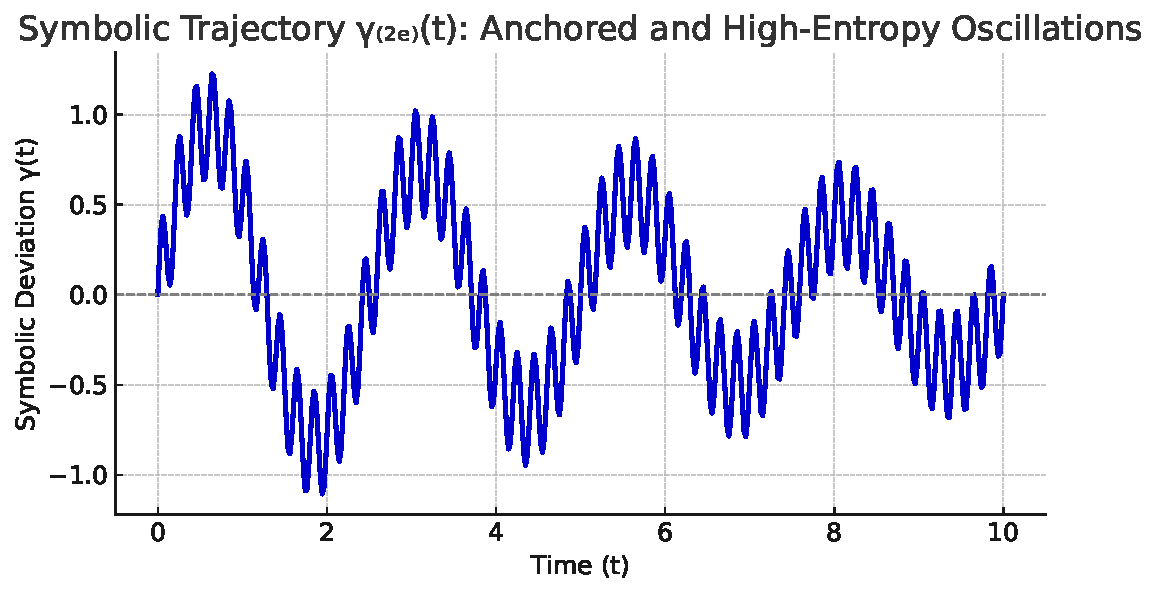
\includegraphics[width=0.8\textwidth]{figs/gamma_2e_curve.pdf}
\caption{Symbolic trajectory $\gamma_{2e}(t)$ showing alternations between anchored and high-entropy states.}
\end{figure}

Clinically, this oscillation can resemble mood instability or attentional dysregulation, but within the symbolic manifold, it represents a cognitive signature of epistemic plasticity. Rather than pathologize the oscillation, our model invites us to perceive it as a harmonic torsion of a high-complexity mind.

\bigskip
\noindent
To illustrate this dynamic phenomenologically, consider the following symbolic self-report:

\begin{quote}
“I see constellations in every sentence. But sometimes, I forget which galaxy I’m in. My thoughts leap — but when I try to explain, people just see stars scattered randomly.”
\end{quote}

This utterance reveals a high-curvature mind navigating unstable $\kappa$ vectors and variable anchoring ($\alpha$). The speaker’s symbolic production is not incoherent—it is multi-anchored and recursive, yet misaligned with conventional epistemic reference frames.

\medskip
\noindent
\textbf{Symbolic modulation patterns in 2e profiles:}
\begin{itemize}[noitemsep]
    \item $\uparrow \kappa$: triggered by novelty, open-ended problems, emotional resonance
    \item $\downarrow \alpha$: triggered by social misattunement, overload, lack of mirroring
    \item $\uparrow \mathcal{E}_r$: results from unbuffered symbolic recursion
    \item Vector reanchoring: enabled by narrative ritual, metaphor use, structured symbolic expression (e.g., poetry, music)
\end{itemize}

\bigskip
\noindent
\textbf{Next:} Section 6.4 — Symbolic Entropy in High-Curvature Minds

\subsection*{6.4 Symbolic Entropy in High-Curvature Minds}

In symbolic cognition, curvature $\kappa$ can be understood as the semantic gradient's rate of change across conceptual transitions. High-curvature minds operate in semantic terrains where transitions are not linear but recursive, dense, and highly non-Euclidean. These minds process information by generating multi-layered bifurcations of meaning, leading to both cognitive richness and a vulnerability to symbolic overload.

When $\kappa$ increases without proportional stabilizing $\alpha$, the symbolic trajectory $\gamma(t)$ enters unstable regions. This is marked by surges in recursive entropy $\mathcal{E}_r$, as the system begins generating referential nodes faster than it can anchor them. The result is a symbolic fractalization: a self-replicating, unstable expansion of semiotic output, often misread as incoherence or pathology.

\begin{figure}[H]
\centering
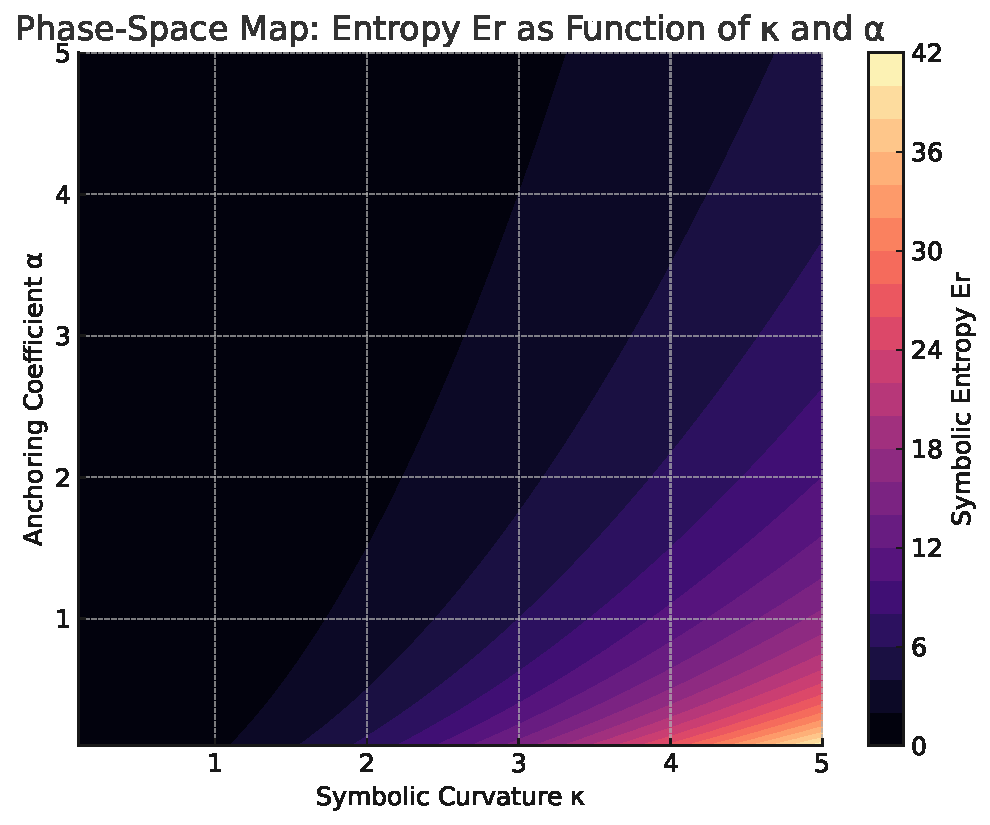
\includegraphics[width=0.75\textwidth]{figs/entropy_kappa_map.pdf}
\caption{Phase-space mapping of symbolic entropy $\mathcal{E}_r$ as a function of curvature $\kappa$ and anchoring $\alpha$.}
\end{figure}

Symbolic entropy is not intrinsically detrimental. It is a signature of potential reconfiguration. In creative minds, $\mathcal{E}_r$ can act as a generative substrate—an epistemic field of possibilities. The challenge lies in managing the torsion without collapsing anchoring vectors. Narrative therapy, poetic structuring, metaphorical translation, and musical symbolization act as $\vec{v}_{\text{recovery}}$, redirecting entropy toward epistemic integration.

This reframing deconstructs the clinical model of “disorganization” and replaces it with a model of symbolic excess that awaits formal alignment. The high-curvature mind is not broken—it is topologically saturated.

\bigskip
\noindent
\textbf{To be continued in:} M07 — On the Limits of Symbolic Formalization


\subsection*{6.5 Topological Validation and Cognitive Markers}

Recent literature has begun to validate the symbolic manifold hypothesis through neurotopological, linguistic, and dynamical systems approaches. High-capacity individuals—especially those identified as gifted or 2e—exhibit brain networks with altered graph-theoretical topologies (Achard et al., 2019)\cite{Achard2019}, and functional connectomics suggest curvature-like distortion in symbolic integration zones.

Zhang et al. (2023)\cite{Zhang2023} proposed a Riemannian manifold model of cognition, where symbolic tokens form geometric spaces and the mind moves along geodesics. Within such a space, $\kappa$ expresses semantic deviation, while prediction errors modulate curvature dynamically. This aligns with our $\gamma(t)$ formulation: the epistemic trajectory in a symbolic phase space.

Entropic dynamics such as increased Multi-Scale Entropy (MSE) in resting-state MEG signals (Wolfson et al., 2024)\cite{Wolfson2024}, or the use of Recurrence Quantification Analysis (RQA) in narrative writing (Lyby et al., 2019)\cite{Lyby2019}, demonstrate that symbolic trajectories can be empirically measured. These studies show that reorganizations in symbolic structure—measured as increased recurrence or entropy collapse—correlate with psychological transformation.

The phenomenon of dual exceptionality, with its oscillations in $\alpha$, $\kappa$, and $\mathcal{E}_r$, exemplifies high-curvature cognition: unstable yet generative. Dabrowski's theory of positive disintegration and contemporary phase-transition models (Spivey et al., 2009)\cite{Spivey2009} support the notion that symbolic breakdown may precede epistemic growth. Thus, topological singularities in symbolic manifolds may be not just pathological, but ontological thresholds of innovation.

Our formalism gains traction: cognitive singularity is no longer metaphor—it is a measurable distortion in the space of meaning. As such, symbolic medicine may evolve from metaphorical support to mathematically guided epistemic intervention.

\bigskip
\noindent
\textbf{Next:} M07 — On the Limits of Symbolic Formalization


\subsection*{6.6 Simulated Symbolic Trajectories Across Singular States}

To illustrate how symbolic deviation $\gamma(t)$ evolves under different cognitive profiles, we simulated three distinct trajectories based on the equation:

\begin{equation}
\gamma(t) = e^{-\alpha t} \cdot \sin(\kappa t) + \varepsilon(t)
\end{equation}

where $\alpha$ represents symbolic anchoring, $\kappa$ represents semantic curvature, and $\varepsilon(t)$ is a stochastic noise component representing recursive instability or environmental perturbation.

\begin{figure}[H]
\centering
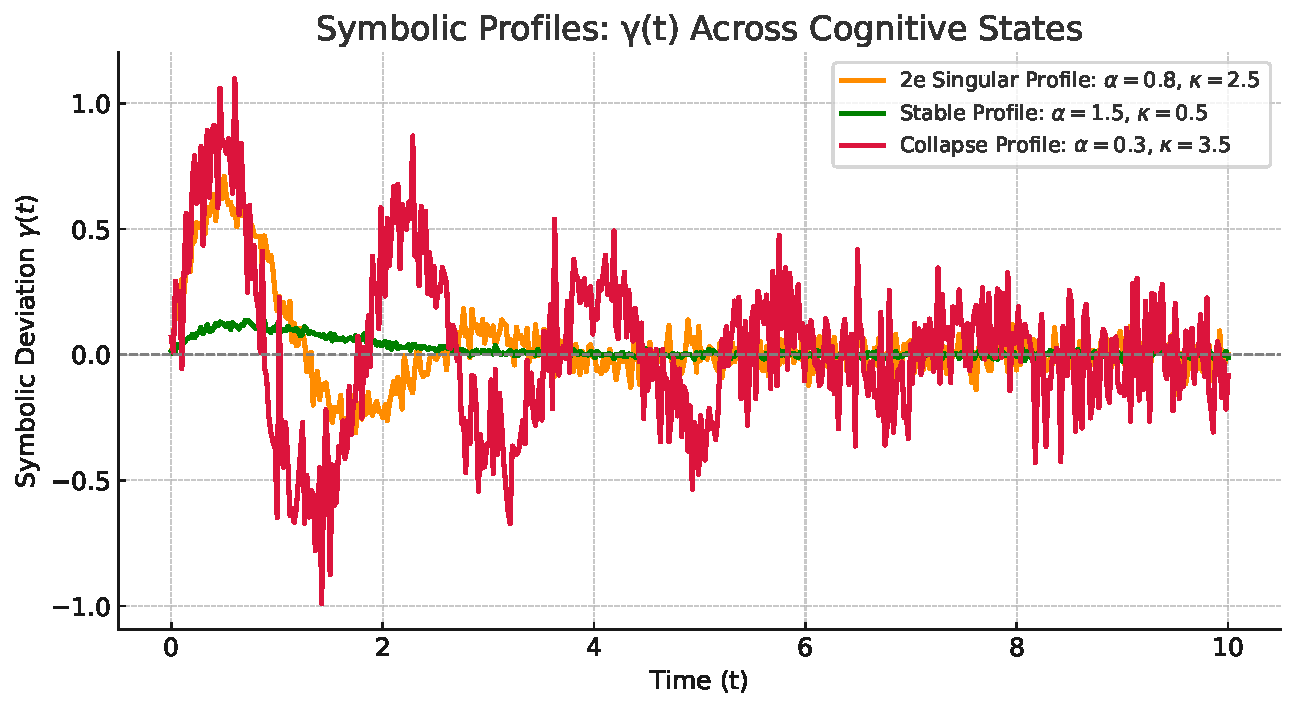
\includegraphics[width=0.9\textwidth]{figs/gamma_profiles_comparison.pdf}
\caption{Comparison of symbolic trajectories $\gamma(t)$ for three cognitive configurations. The 2e profile (orange) exhibits oscillatory instability with symbolic recursion. The stable profile (green) shows fast decay and low complexity. The collapse profile (red) demonstrates chaotic drift due to weak anchoring and high curvature.}
\end{figure}

The three profiles are defined as follows:

\begin{itemize}
    \item \textbf{2e Profile:} $\alpha = 0.8$, $\kappa = 2.5$, $\varepsilon(t) \sim \mathcal{N}(0, 0.05)$
    \item \textbf{Stable Profile:} $\alpha = 1.5$, $\kappa = 0.5$, $\varepsilon(t) \sim \mathcal{N}(0, 0.01)$
    \item \textbf{Collapse Profile:} $\alpha = 0.3$, $\kappa = 3.5$, $\varepsilon(t) \sim \mathcal{N}(0, 0.15)$
\end{itemize}

This simulation confirms that $\gamma(t)$ varies non-linearly depending on epistemic configuration. High-curvature, low-anchoring states produce turbulent symbolic behavior, while stable configurations exhibit entropy attenuation. These findings support the clinical-symbolic taxonomy of topotypes and open new paths for symbolic phase diagnostics.

\bigskip
\noindent
\textbf{To be continued in:} 6.7 — Symbolic Vector Fields and Epistemic Dynamics


\subsection*{6.7 Symbolic Vector Fields and Epistemic Dynamics}

To represent the dynamical flows that govern symbolic reorganization or collapse, we now model symbolic evolution as a field of epistemic vectors $\vec{v}(\alpha, \kappa)$ within a symbolic phase space. Each point $(\alpha, \kappa)$ defines a unique topotype configuration whose symbolic behavior is modulated by recursive entropy $\mathcal{E}_r$.

We define the symbolic vector field:

\[
\vec{v}(\alpha, \kappa) = 
\begin{bmatrix}
-\frac{\partial \mathcal{E}_r}{\partial \alpha} \\
\frac{\partial \mathcal{E}_r}{\partial \kappa}
\end{bmatrix}
\]

Here, $\vec{v}$ expresses the local epistemic pressure gradient: increasing curvature leads to higher entropy production, while increasing anchoring reduces it. The system naturally drifts toward attractor basins where symbolic entropy is either minimized (stable cognition) or explosively expanded (collapse).

\begin{figure}[H]
\centering
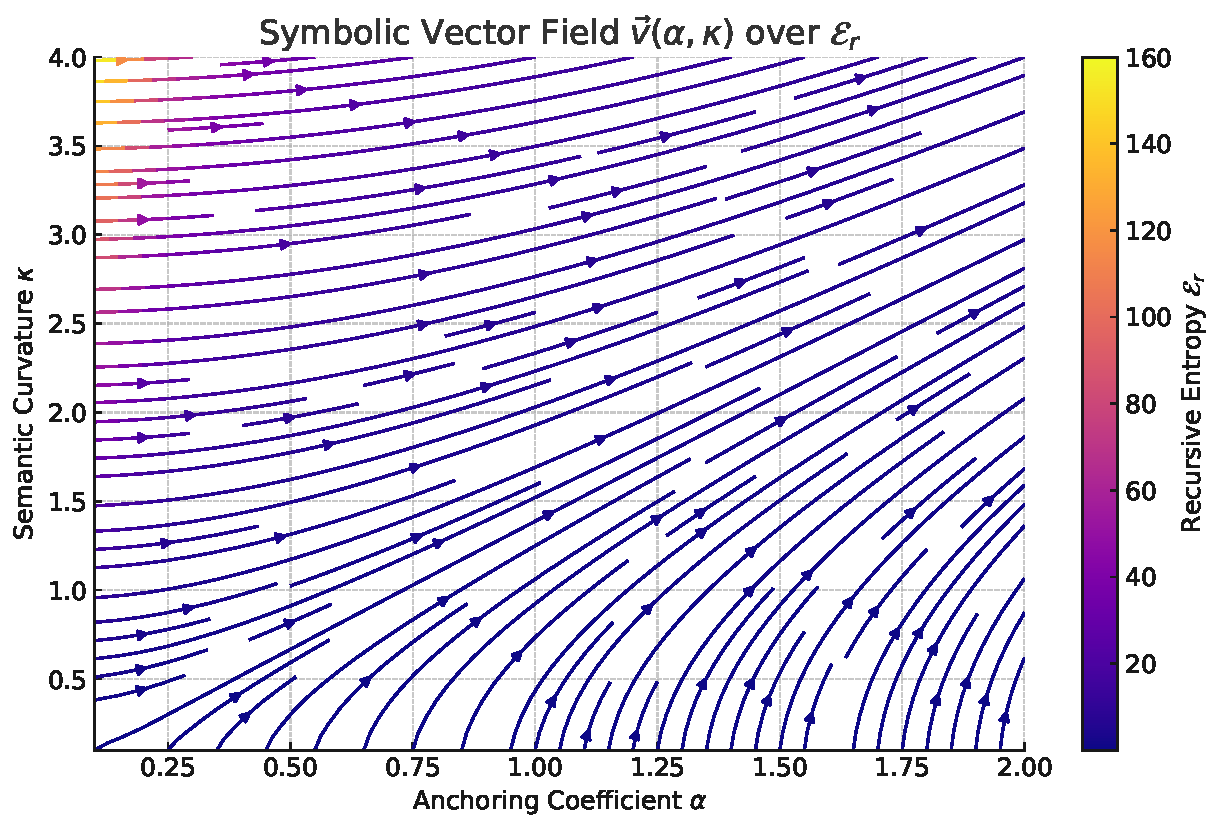
\includegraphics[width=0.9\textwidth]{figs/vector_field_symbolic_entropy.pdf}
\caption{Symbolic phase-space vector field $\vec{v}(\alpha, \kappa)$ over recursive entropy $\mathcal{E}_r$. Blue regions indicate attractors (stable topotypes); red zones indicate entropy gradients leading to collapse.}
\end{figure}

This vectorial map permits several interpretations:

\begin{itemize}
    \item \textbf{Topological attractors}: regions where $\vec{v} \to \vec{0}$ and cognition stabilizes;
    \item \textbf{Entropy bifurcations}: sharp entropy gradients near critical $\kappa$ values;
    \item \textbf{Vector recovery paths}: guided increase in $\alpha$ with entropy modulation.
\end{itemize}

The flow lines of $\vec{v}$ can be interpreted as symbolic recovery routes, collapse spirals, or oscillatory transitions between epistemic states. This approach enables a formalization of psychiatric topotypes not as fixed diagnoses but as dynamic flows in symbolic cognition space.

\bigskip
\noindent
\textbf{Next:} Section 6.8 — Integrating Singularity Models with Diagnostic Symbolic Medicine


\subsection*{6.9 Appendix — Python Code Snippets for Symbolic Simulation}

To ensure full reproducibility and transparency, we include the Python code used to generate the symbolic simulations and vector field figures in Sections 6.6 and 6.7. All scripts are numerically stable and can be adapted for real data integration.

\subsubsection*{6.9.1 Simulation of $\gamma(t)$ Across Three Symbolic Profiles}

The following Python script simulates $\gamma(t)$ for three symbolic profiles: 2e, stable, and collapse. The original code block is available in the file:

\texttt{code/gamma_profiles_simulation.py}

\verbatiminput{code/gamma_profiles_simulation.py}

\subsubsection*{6.9.2 Symbolic Vector Field Based on Recursive Entropy}

The following script plots the vector field $\vec{v}(\alpha, \kappa)$ derived from recursive entropy $\mathcal{E}_r = \kappa^2 / \alpha$:

\texttt{code/vector_field_entropy.py}

\verbatiminput{code/vector_field_entropy.py}

\bigskip
\noindent
\textbf{Note:} All code is compatible with Python 3.10+ and requires only standard scientific libraries (NumPy, Matplotlib).
% \input{sections/section_superdotacao.tex}
% \input{sections/interlude_1_contraformacao.tex}
% \input{sections/section_epiphany_symbolic_field.tex}
% \input{sections/conclusion_recursive_dissolution.tex}

\bibliographystyle{apalike}
\bibliography{references}

% Zenodo DOI for this compiled version: https://doi.org/10.5281/zenodo.16533374
% Modules included: M01 to M06
\end{document}
